% Chapter 3

\chapter{Metodo per il ranking delle stazioni ferroviarie} % Chapter title

\label{ch:mathtest} % For referencing the chapter elsewhere, use \autoref{ch:mathtest}

Il fine del metodo che ci si accinge a descrivere è valutare il livello di rischio frana (Exposure) al quale potrebbero essere soggetti un insieme di assets. Con tale valutazione si potrà creare una graduatoria degli assets più a rischio di una determinata zona (\textit{GeoArea}) e potrà essere di supporto agli enti responsabili di manutenzione o controllo della zona stessa. Il metodo che verrà sviluppato tiene a mente tutte le considerazioni presentate nella introduzione, da cui è emerso che oltre alla ripidità del pendio e allo spazio percorso dalla frana è fondamentale anche la traiettoria seguita. Quest'ultima è alla base del metodo ed è stato il principale elemento di studio. Per un'analisi approfondita di questi aspetti sono sono state introdotte le curve di livello ($\mathcal{I}$). Inoltre il territorio preso in considerazione (\textit{GeoArea}), dove sono dislocati gli assets strategici ($\mathcal{B}$), è stato suddiviso in piccole particelle di terreno ($\mathcal{Z}$) dalle quali può aver origine una frana se si verificano determinate condizioni che andremo a definire.


\begin{figure}[h]
	\centering
	\includegraphics[width=0.7\textwidth]{images/raggio_di_azione_frana}
	\caption{Due assets che si trovano nei pressi di un pendio. Entrambi hanno la propria \textit{HazardArea} di raggio $r$, di cui quella dell'edificio in rosso comprende il punto di distacco del masso. Quindi l'edificio si trova in una zona pericolosa, al contrario di quello di colore verde. }
	\label{raggio_azione_frana}
\end{figure}

Il metodo calcola per ogni asset $b_i$, il relativo valore di exposure. Ricordando dall'introduzione che una frana può estendersi per una distanza notevole ma pur sempre limitata (Figure \ref{raggio_azione_frana}), sembra logico limitare l'area di studio alla sola ($HazardArea_i$). L'analisi che segue quindi interesserà le sole Zones $\mathcal{Z}$ all'interno di tale area, ovvero le particelle appartenenti all'insieme $\mathcal{NZ}_i$ (\textit{Nearest Zones} di $b_i$) (Figura \ref{landslide0}).
Come detto in precedenza, elemento fondamentale alla base del metodo è la  traiettoria di frana. Il metodo infatti stima tale traiettoria per ognuna delle \textit{Nearest Zones} $nz_{i,j} \in \mathcal{NZ}_i$ dunque è indispensabile considerare le curve di livello  (Figura \ref{landslide1}). 

\begin{figure}[h]
	\hspace{0.05\linewidth}
	\begin{minipage}[t]{0.4\linewidth}
		\centering
		\includegraphics[width=\textwidth]{images/landslide0}
		\caption{In giallo è evidenziata una delle Nearest Zone dell'edificio di colore rosso.}
		\label{landslide0}
	\end{minipage}
	\hspace{0.05\linewidth}
	\begin{minipage}[t]{0.4\linewidth}
		\centering
		\includegraphics[width=\textwidth]{images/landslide1}
		\caption{Impiego delle curve di livello per il calcolo della traiettoria della frana}
		\label{landslide1}
	\end{minipage}
\end{figure}

Naturalmente le sole curve di livello di interesse alla $nz_{i,j}$ sono quelle che intersecano la $HazardArea_i$, ovvero le (Nearest Isoipses) $\mathcal{NI}_i$.
Queste ultime vengono utilizzate per determinare la distribuzione delle masse all'interno della particella di terreno $nz_{i,j}$. Pertanto esse verranno utilizzate per frazionare la $nz_{i,j}$  in frammenti $zf_{i,j,t}$. I centri di massa ($czf_{i,j,t}$) di tali frammenti sono alla base del calcolo della regressione lineare. Dal calcolo della regressione lineare otteniamo la retta ($lr_{i,j}$) che stima appunto la traiettoria di frana della particella $nz_{i,j}$. 

A questo punto, ricavata la retta che stima la traiettoria di frana $lr_{i,j}$ della particella $nz_{i,j}$, bisogna determinare se la presunta frana di tale particella "impatta" o meno sull'edificio $b_i$ oggetto di analisi. Per poter comprendere appieno cosa si intende per "impatto" è necessario definire le seguenti notazioni:

\begin{enumerate}
	\setcounter{enumi}{13}
	\item \textbf{$ \mathcal{BLR}_i $} (\textbf{Buffered Linear Regressions}) $= \{blr_{i,j}(i=1,..,\mathbf{card}(\mathcal{B})),(j=1,..,\mathbf{card}(\mathcal{NZ}_i)\}$ | $\forall lr_{i,j} \in $ \textbf{$ \mathcal{LR}_i $} si ha che $blr_{i,j}$ è la geometria risultante dalla \textit{LineBuffering} di $lr_{i,j}$. $blr_{i,j}$ rappresenta quella che potrebbe essere la scia della frana di $nz_{i,j}$ alla quale ci si riferisce. Ovvero identifica l'area che tale frana mette a rischio. 
	Per una migliore comprensione riferirsi alla (Figura \ref{buffer_regression})
	
	\begin{figure}[h]
		\centering
		\includegraphics[width=0.5\textwidth]{images/buffer_rect}
		\caption{La \textbf{Buffered Linear Regression} $blr_{i,j}$ ottenuta dalla \textit{LineBuffering} della retta di regressione lineare $lr_{i,j}$. Essa rappresenta l'area attorno alla retta entro una distanza $d$ dalla stessa.}
		\label{buffer_regression}
	\end{figure}
	
	\item \textbf{$ \mathcal{LS}_i $} (\textbf{LandSlides}) $ = \{ls_{i,j}(i=1,..,\mathbf{card}(\mathcal{B})),(j=1,..,\mathbf{card}(\mathcal{LS}_i)\}$ con $\mathcal{LS}_i \subseteq \mathcal{BLR}_i$  sottoinsieme | $\mathcal{LS}_i = (\mathcal{BLR}_i  \cap BuildingBuffer_i)	\not= \emptyset $.
	Con parole esplicite, gli elementi dell'insieme $ \mathcal{LS}_i $ sono	le sole $blr_{i,j}$ che intersecano il \textit{BuildingBuffer$_i$}. Nello specifico, le sole frane che "impattano" l'edificio $b_i$ (Figura \ref{landslides}).
	
	\begin{figure}[h]
		\centering
		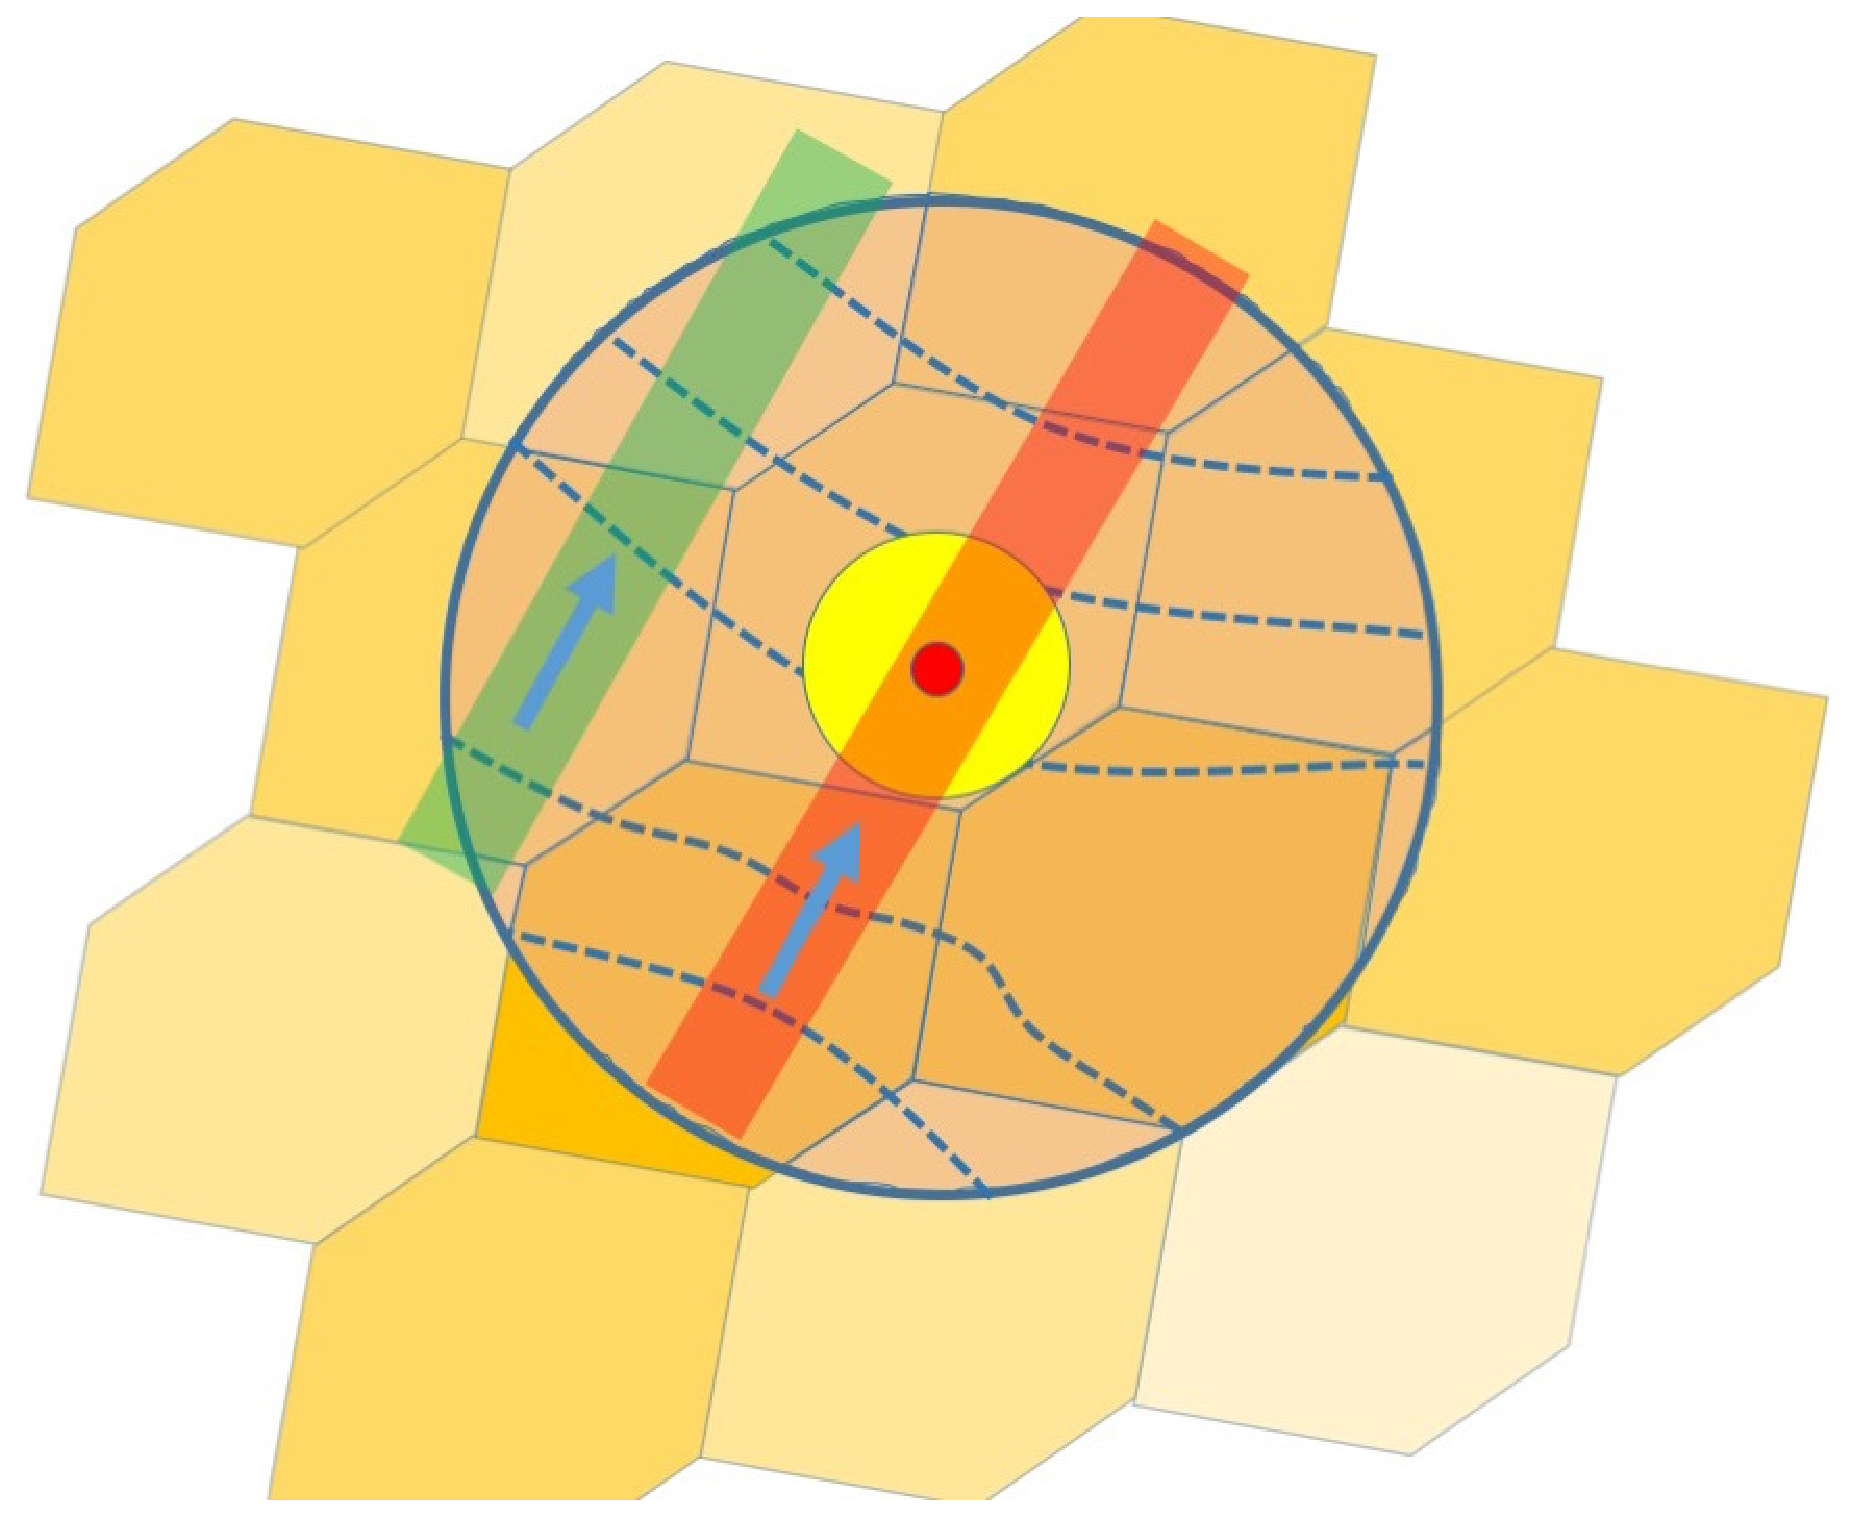
\includegraphics[width=0.4\textwidth]{images/landslides}
		\caption{Il rettangolo verde rappresenta una \textit{Buffered Linear Regression} che non costituisce un pericolo per l'edificio. In rosso invece è stata raffigurata una \textit{Buffered Linear Regression} che impatta sull'edificio pertanto essa appartiene all'insieme $\mathcal{LS}_i$ del relativo building $b_i$.}
	\label{landslides}
	\end{figure}
	

%\begin{figure}[h]
%	\hspace{0.05\linewidth}
%	\begin{minipage}[t]{0.4\linewidth}
%		\centering
%		\includegraphics[width=\textwidth]{images/landslide2}
%		\caption{Modificare immagne cn landslide che pasa affianco alla stazione}
%		\label{landslide2}
%	\end{minipage}
%	\hspace{0.05\linewidth}
%	\begin{minipage}[t]{0.4\linewidth}
%		\centering
%		\includegraphics[width=\textwidth]{images/landslide3}
%			\caption{textcolor{red}{Da scrivere}}
%		\label{landslide3}
%	\end{minipage}
%\end{figure}
	
\end{enumerate}

Avendo definito la nozione di frana che "impatta" sull'edificio $b_i$, rimane da tener conto di un altro fattore determinante, ossia l'entità di tale "impatto". Una \textit{LandSlide} di fatto può "impattare" su un edificio in modo totale o parziale e di conseguenza influire diversamente sul valore di exposure della stessa. Introduciamo pertanto la notazione di \textit{Impact Factor}

\begin{enumerate}
	\setcounter{enumi}{15}
	
	\item \textbf{$IFls_{i,j}$} (\textbf{Impact Factor}) è un valore percentuale $\in(0,1]$ che esprime l'entità dell'impatto della $ls_{i,j}$ sull'edificio $b_i$. Essa corrisponde al rapporto tra l'area della $ls_{i,j} \cap BuildingBuffer_i$ e l'area del $BuildingBuffer_i$ (Equazione \ref{eq:impactfactor}). Un valore di $IFls_{i,j}=1$ equivale a dire che la frana impatta in modo totale sull'edificio. Da tenere conto che un valore pari a 0 non è possibile essendo l'insieme $ \mathcal{LS}_i $ quello delle sole frane che impattano su $b_i$.
	
	\begin{equation}\label{eq:impactfactor}
	ImpactFactor=\frac{Area(BuildingBuffer_i \cap ls_{i,j})}{Area(BuildingBuffer_i)}
	\end{equation}
	
	In (Figura \ref{impact_factor}) vediamo da due diverse prospettive i casi di impatto di una \textit{LandSlide}.
	
	\begin{figure}[h]
		\centering
		\includegraphics[width=0.9\textwidth]{images/landslide5}
		\caption{A sinistra il caso di impatto totale a cui corrisponderà una \textit{Impact Factor} pari a 1. A destra il caso di impatto parziale a cui corrisponderà una \textit{Impact Factor} $<1$  }
		\label{impact_factor}
	\end{figure}
	
\end{enumerate}

\newpage 
A questo punto si ha tutto il necessario per poter calcolare l'exposure dell'edificio $b_i$ che naturalmente terrà conto di tutti i fattori descritti in precedenza. Quindi, per ogni $b_i$ l'Exposure sarà calcolata come la somma dei valori di exposure parziali $Pexp_{i,j}$ (Definizione \ref{Pexp}) derivanti dai contributi delle sole \textit{NearestZones} le quali \textit{LandSlides} $ls_{i,j}$ impattano sull'edificio stesso.
Definiamo tali zone come \textit{LandSlideZones} (Definizione \ref{LSZ})

\begin{enumerate}
	\setcounter{enumi}{16}

	\item \label{LSZ} \textbf{$ \mathcal{LSZ}_i $ (LandSlideZones)} $ = \{lsz_{i,j}(i=1,..,\mathbf{card}(\mathcal{B})),(j=1,..,\mathbf{card}(\mathcal{LSZ}_i)\}$ con $\mathcal{LSZ}_i \subseteq \mathcal{NZ}_i$ | $\mathcal{LSZ}_i$ 
	è l'insieme delle sole $nz_{i,j}$ aventi $ls_{i,j}$ che impattano sull'edificio $b_i$. 
	Con parole più esplicite, $lsz_{i,j}$ è la Zone relativa alla \textit{LandSlide} $ls_{i,j}$. 
	Tenendo presente che $\mathcal{LSZ}_i$ è un sottoinsieme di $\mathcal{NZ}_i$, l'elemento $lsz_{i,j}$  è descritto dalla medesima tupla <\textit{ID}, \textit{boundary}, \textit{$Sz_k$}> di $nz_{i,j}$ . 
	
	\item \label{Pexp} $pexp_{i,j}$ \textbf{(Partial Exposure)} | $ pexp_{i,j}(i=1,..,\mathbf{card}(\mathcal{B})),(j=1,..,\mathbf{card}(\mathcal{LSZ}_i)$ è il valore di exposure parziale con cui la \textit{LandSlideZone} $lsz_{i,j}$ influisce sull'edificio $b_i$. Tale valore dipende dal valore di $Sz_k$ della $lsz_{i,j}$ , dall'area della zone stessa, e dal \textit{Impact Factor} $IFls_{i,j}$ della relativa \textit{LandSlide} sull'edificio $b_i$. Matematicamente $pexp_{i,j}$ è descritta dalla (Equazione \ref{eq:exposure2}). Nel caso singolare in cui ($lsz_{i,j}$ contiene $b_i==true$), ovvero quando si sta calcolando la \textit{Partial Exposure} della specifica \textit{LandSlideZone} che contiene $b_i$, la relativa $pexp_{i,j}$ viene calcolata imponendo la $IFls_{i,j}=1$ (Equazione \ref{eq:exposure3})  
	\\
	\begin{enumerate}
		\item[$\bullet$] Se $lsz_{i,j}$ contiene $b_i$
		\begin{equation}\label{eq:exposure2}
		pexp_{i,j} =(Area)*(Sz_{k}) * IFls_{i,j}
		\end{equation}
		
		\item[$\bullet$] Altrimenti
		\begin{equation}\label{eq:exposure3}
		pexp_{i,j} =(Area)*(Sz_{k})
		\end{equation}
	\end{enumerate}

	{Con $j$ fissato, "Area" e "$Sz_k$" sono la rispettiva Area e valore $Sz_k$ della relativa $lsz_{i,j}$.}
	
\end{enumerate}

Pertanto abbiamo che l'exposure totale risulta essere definita dalla seguente equazione

\begin{equation}\label{eq:exposure1}
exp_i =\sum_{j=1}^n pexp_{i,j}
\end{equation}

ove n=$\mathbf{card}(\mathcal{LSZ}_i)$
\bigbreak

Infine il metodo restituirà per ogni edificio $b_i$ della \textit{GeoArea} un valore di exposure $exp_i$.






